\section{Scalar field and friends}

\subsection*{Overview}

A scalar field \(f\) from \(\mathbb R^2 \to \mathbb R\) can be visualized by a surface in three dimensions. On this surface, the x-traces and y-traces can be shown as strings lying on the surface. The partial-derivatives can be show as vector stangent to each trace. The gradient is a vector that points in the direction of steepest descent. Level sets can be depicted as lines going around the surface. It can be noted visually that the gradient is always perpendicular to the level set. \cite{field6}

\subsection*{Theoretical Basis}

This time, the maths are relatively straightforward.

% The level set locally is given at the point 

\subsection*{Implementation details}

We created seven different virtual objects. In order to demonstrate the fact that gradient vectors point in the direction of greatest descent, we generated \verb+gradFieldR+ and overlaid it upon the graph of a scalar field, \verb+fieldR+, using \href{https://reference.wolfram.com/language/ref/Plot3D.html}{Plot3D}. The surface is semi translucent in order to be able to view the slices of x and y as separate functions. Next, we revealed that the gradients are always perpendicular to the level sets by using a mesh function in order to display slices of the function at varying values of Z that are constant along each slice. The x-trace is done by holding y constant. This creates the parametric \verb+{x, ymid, field /. y-> ymid}+ as a function of \verb+x+. This is rendered with \href{https://reference.wolfram.com/language/ref/ParametricPlot3D.html}{ParametricPlot3D}. Then the vector $\langle 1, 0, \frac{\partial f}{\partial x} \rangle$ is depicted eminating from $\langle x, y, f(x, y) \rangle$. The x partial is green and the y is red. Finally, the gradient is drawn from a point on the graph that is evaluated from.

\subsection*{Usage notes}

This model can be used to demonstrate topics that we learned in both the second and third six weeks of multivariable. Students will no longer have to worry about imaginary mountains demonstrations with this visual included in lectures. The slices no longer have to be silly putty or moon sand in the shape of functions, but instead actual 2-dimensional functions displayed on the graph. Any point and any surface can be chosen to displayed, all the calculations will be automatic, and the vectors will always be generated (except for at singularities if they exist).

These visualizations can be used in lectures 11 Partial Derivatives,12, Derivatives continued, and 15 Gradients and Directional Derivatives

\begin{enumerate}
\item The variable \verb+fieldF+ is the scalar valued function that can be altered to fit any function of your choice. 
\item \verb+xmin, xmax, ymin, ymax+ are the domain boundaries which can also be changed to preference.
\item \verb+xint, yint+ represents the increments for the display of the gradient vector field (also known as the spacing between the vectors).
\item \verb+xmid, ymid+ are the point at which the gradient vector, x partial, y partial, and x and y slices are calculated and displayed at. 
\item All of these variables are free to edit and the program will accommodate to new models of choice. 
\end{enumerate}

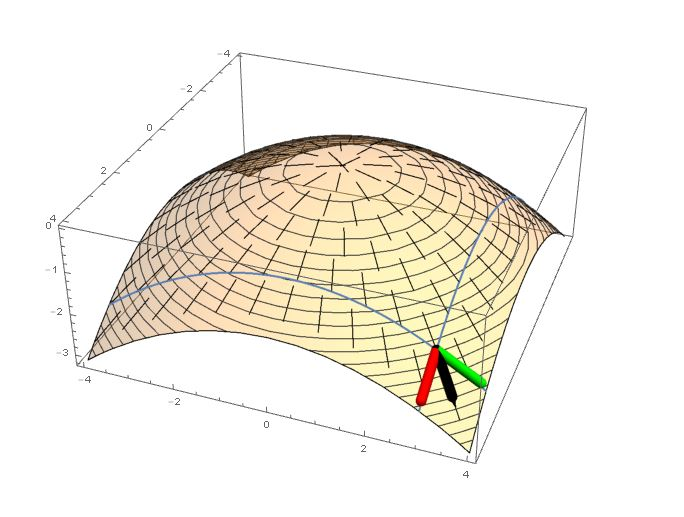
\includegraphics[height=10cm]{../exhibit/field.jpg}

%%% Local Variables:
%%% mode: latex
%%% TeX-master: "main"
%%% End:
